\documentclass[12pt,letterpaper,norsk]{article}
\usepackage{babel}
\usepackage[T1]{fontenc}
\usepackage{extsizes}
\usepackage{graphicx}
\usepackage[bookmarks]{hyperref}
\usepackage{pdfpages}
\usepackage[lyric]{songs}
\usepackage{tikz}
\usepackage[utf8]{inputenc}

\title{Sanghefte 17. mai 2017}
\author{Joakim Lindqusiter}
\date{}

\setlength{\oddsidemargin}{0in}
\setlength{\evensidemargin}{0in}
\setlength{\textwidth}{6in}
\setlength{\topmargin}{0in}
\setlength{\topskip}{0in}
\setlength{\headheight}{0in}
\setlength{\headsep}{0in}
\setlength{\textheight}{9.1in}
\settowidth{\versenumwidth}{1.\ }

\renewcommand*{\familydefault}{\ttdefault}

\newindex{titleidx}{lbtitle}
\newauthorindex{authidx}{lbauth}
\newscripindex{scripidx}{lbscrip}

\makeatletter
\renewcommand\beginsong[1]{%
	\ifSB@insong\SB@errboo\SB@closeall\fi%
	\ifSB@intersong\SB@errbor\SB@closeall\fi%
	\SB@insongtrue%
	\def\SB@closeall{\endsong}%
	\SB@parsetitles{#1}%
	\global\setbox\SB@songwrites\box\voidb@x%
	\SB@clearbskeys%
	\@ifnextchar[\SB@bskvfmt\SB@@beginsong%
	\hypersetup{bookmarksdepth=0}%
	\phantomsection%
	\addcontentsline{toc}{subsection}{\numberline{\thesongnum}#1}%
	\hypersetup{bookmarksdepth=2}%
}
\makeatother

\usetikzlibrary{shapes,arrows}

\tikzstyle{decision} = [diamond, draw, fill=blue!20, text width=1in, text badly centered, node distance=1.8in, inner sep=0pt]
\tikzstyle{block} = [rectangle, draw, fill=blue!20, text width=5em, text centered, rounded corners, minimum height=1in, node distance=1.8in]
\tikzstyle{line} = [draw, -latex']
\tikzstyle{cloud} = [draw, ellipse, fill=red!20, node distance=1in, minimum height=2em]

\begin{document}

\newpage

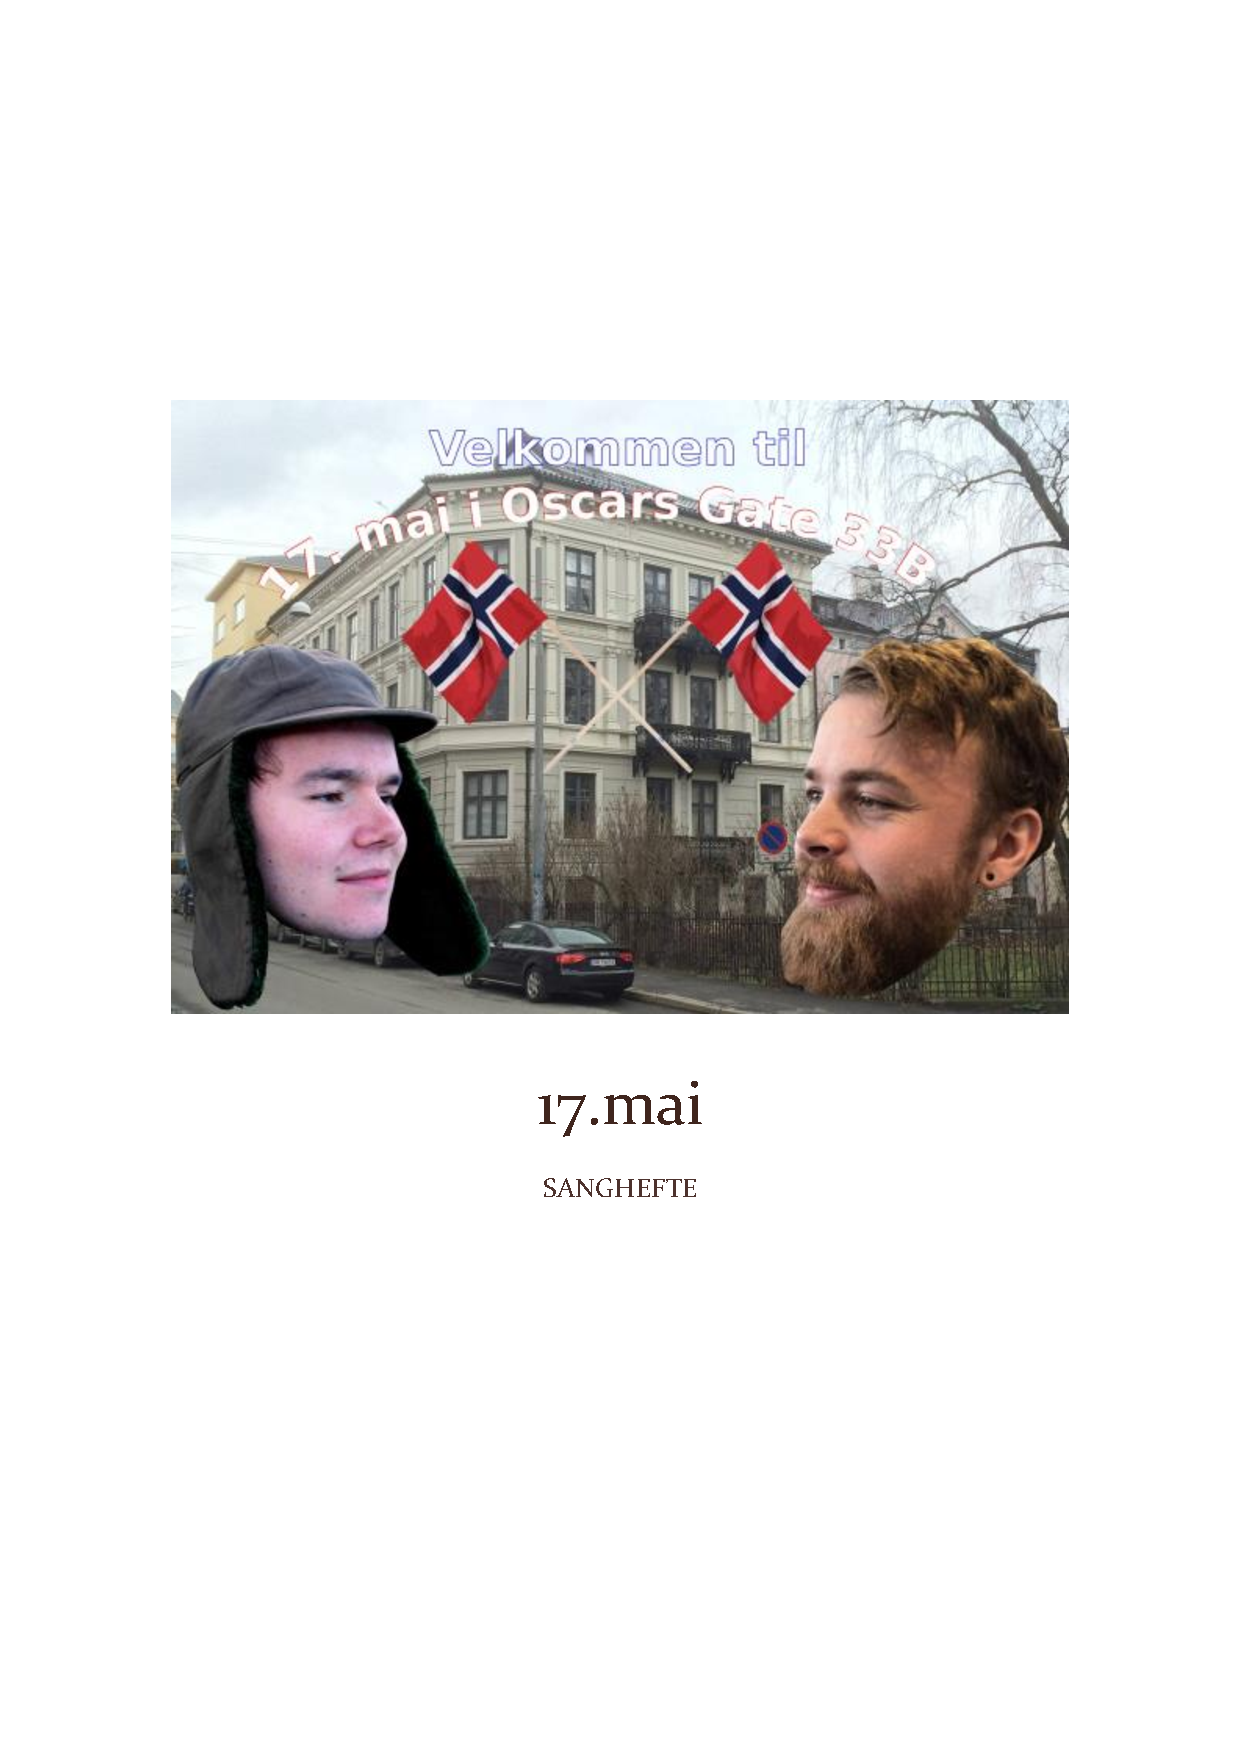
\includepdf{forside_17mai.pdf}
\newpage

\tableofcontents


\begin{songs}{titleidx,authidx,scripidx}

\beginsong{Norge i rødt, hvitt og blått}
\beginverse
Hvorhen du går i li og fjell,
en vinterdag, en sommerkveld
med fjord og fossevell,
fra eng og mo med furutrær
fra havets bryn med fiskevær
og til de hvite skjær,
møter du landet i trefarvet drakt,
svøpt i et gjenskinn av flaggets farveprakt.
Se, en hvitstammet bjerk oppi heien,
rammer stripen med blåklokker inn
mot den rødmalte stuen ved veien,
det er flagget som vaier i vind.
Ja, så hvit som det hvite er sneen,
og det røde har kveldssolen fått,
og det blå ga sin farve til breen,
det er Norge i rødt, hvitt og blått.
\endverse

\endsong

\end{songs}

\newpage


\end{document}
